%!TEX root = ../dissertation.tex

\chapter{Knowledge Enhanced Neural Networks}\label{chapt:kenn}
%TODO: rivedere la presentazione di kenn.... dire a che classe di NSI appartiene

%TODO CORREGGERE ERRORI segnalati da Alessandro
Knowledge Enhanced Neural Networks (KENN) \cite{daniele2019kenn} is a special type of Neural Network (NN) layer, designed for injecting logical knowledge into a pre-existing base NN. More specifically, it is a residual layer designed to be stacked after the last layer of a standard NN, in order to boost its predictive performances via the addition of a Prior Knowledge in the form of first order logic clauses. In this chapter we will describe the theory behind KENN, its architecture, and experimental results.

\section{Theoretical Framework}\label{sec:theoretical_framework}
 We present here the theoretical framework behind KENN. The first step will be to rigorously define the symbolic language and how to link it with the theoretical framework of NNs, which consists in defining a semantic for the language. Next, we will describe the process with which the truth value of a clause can be increased, and how to integrate this method inside NNs.
 
 \subsection{Prior Knowledge and language semantic}

\begin{definition}[Prior Knowledge]
	Collection of formulas of a function-free FO language $\mathcal{L}$ whose signature is defined with a set of constants $\mathcal{C} = \{a_1, \dots, a_l\}$ and a set of predicates $\mathcal{P} = \{p_1, \dots, p_q\}$. Each predicate can be applied to a specific number of constants $n$, which we will define as the \textit{arity} of the predicate.
\end{definition}

\begin{definition}[Clause]
	A clause is defined to be of the following form:
	\begin{equation}
	c := \bigvee_{i=1}^k l_i, \quad l_i \neq l_j \quad \forall i \neq j.
	\end{equation}
	where $l_i$ is a literal, i.e. a formula constituted only by a $n$-ary predicate, or its negation. Also clauses have an arity, which is by definition the maximum arity of the predicates that constitute it.
\end{definition}

One example of a clause could be the following: 
\begin{equation}
c(x,y) = \neg Smoker(x) \vee \neg Friends(x,y) \vee Smoker(y)
\label{example:clause}
\end{equation} which is equivalent to the clause $Smoker(x) \wedge Friends(x,y) \Rightarrow Smoker(y)$, but expressed as a disjunction of literals. Such a clause is constituted by two predicates: $Smoker(x)$, a unary predicate expressing the statement \say{\textit{$x$ is a smoker}}, and $Friends(x,y)$, a binary predicate which expresses the statement \say{\textit{$x$ and $y$ are friends}}. Therefore, this clause expresses the rule \say{\textit{if $x$ is a smoker and $x$ and $y$ are friends, than also $y$ is a smoker}}. Note that the variables $x$ and $y$ are supposed to be universally quantified, since our aim is to express general knowledge. We now give another definition:

\begin{definition}[Grounding of a clause]
	The grounding of an $n$-ary clause $c$, denoted as \\ $c[x_1/k_1, \dots, x_n/k_n]$,
	is the clause obtained by substituting $k_i$ to $x_i, \forall i=1,\dots,n$.
\end{definition}

Going back to the example of before, assume that $a$ and $b$ are two specific persons. Then, the grounding of clause (~\ref{example:clause}) will be $$c(x/a, y/b) = c(a,b) = \neg Smoker(a) \vee \neg Friends(a,b) \vee Smoker(b).$$

The next step is to build a semantic for the formal language $\mathcal{L}$, that is, how to interpret the symbols that we are working with. In practice, this will consist on defining a way to map constants towards a domain, and predicates to functions that go from such domain to a truth value. To clarify, consider the following example: let $a$ be a constant and let $P$ be a predicate, such that $P(x)$ expresses the statement \say{\textit{$x$ is a prime number}}. In this case, there is a natural way to define an interpretation for our symbols, that is to map constants to the domain of natural numbers and to map $P$ to the function $f: \mathbb{N}\longrightarrow\{0,1\}$, where $f(n)=1$ if $n$ is prime, and $0$ otherwise. Now, we define the semantic of $\mathcal{L}$.

\begin{definition}[Semantic of $\mathcal{L}$]
	The semantic of $\mathcal{L}$ is defined by means of a pair of functions $\left( \mathcal{I}_{\mathcal{C}}, \mathcal{I}_{\mathcal{P}} \right)$, that, together, define an \textit{interpretation} for the symbols of our language and are defined as follows:
	\begin{equation}
	\begin{aligned}[c]
			\mathcal{I}_{\mathcal{C}}: \mathcal{C} &\longrightarrow \mathbb{R}^l\\
			c&\longmapsto x,
	\end{aligned}
	\qquad \qquad
	\begin{aligned}[c]
	\mathcal{I}_{\mathcal{P}}: \mathcal{P} &\longrightarrow \left( \mathbb{R}^{nl} \rightarrow \left[0,1\right] \right)\\
	P &\longmapsto f
	\end{aligned}
	\end{equation}	
	Where $n$ is the arity of the predicate $P$ and $f$ is a function that takes in input the interpretations of $n$ constant symbols, $\mathcal{I}_C(c_1), \dots, \mathcal{I}_C(c_n)$ and returns the truth value of $P(c_1,\dots,c_n)$. Note that, to make the notation lighter, we will omit the subscript when it's clear whether the argument of the interpretation is a literal or a constant term.
\end{definition}

One could already see an analogy with the theoretical setup of NNs. In fact, each constant symbol $c$ is mapped to a $l$-dimensional real vector, which can be seen as the feature vector characterizing the real world object identified by $c$. Another important detail is that the truth value of each literal, in our setup, is not determined by a hard assignment of $0$ or $1$, but is represented by a real number in the interval $\left[ 0,1 \right]$. This is a crucial point: indeed, the truth value in our semantic is trying to represent predictions by a NN, which are always expressed in terms of probability. The natural consequence of this choice is that, from this point on, we will have to rely on the rules of Fuzzy Logic \cite{novak1987first}, which is a generalization of the standard Boolean logic where the truth value of variables can take the value of any real number between $0$ and $1$. 

\subsection{$t$-conorm Functions}
With our definition of a semantic for $\mathcal{L}$, we can now give an interpretation for constants and predicates. The next step is to find a way to interpret clauses, or, more specifically, a way to determine the truth value of a grounded clause. We saw that, by definition, a clause is a disjunction of literals: this means that we only need a way to define the interpretation of a negated predicate and of the disjunction of two predicates. As stated above, since we are allowing truth values in the range $\left[ 0,1\right]$, we will need to use the rules of Fuzzy Logic. For computing the truth value of a negated predicate, the standard way in Fuzzy Logic is to use the Lukasiewicz Negation.

\begin{definition}[Lukasiewicz Negation]
	If $P \in \mathcal{P}$ is a predicate, then:
	\begin{equation}
	\mathcal{I}(\neg P) = 1 -\mathcal{I}(P)\footnote{Writing $1 -\mathcal{I}(P)$ is a slight abuse of notation since $\mathcal{I}(P)$ is a function (or is it?).} 
	%TODO: capire se è abuso di notazione 
	\label{eq:lukasiewicz}
	\end{equation}
		
	
\end{definition}

So for example if the truth value of a predicate is $\mathcal{I}(P)(x) = 0.8$, the truth value of its negated copy would be $\mathcal{I}(\neg P)(x) = 0.2$. It is worth noting that this definition is equivalent to the Boolean negation when $\mathcal{I}(P) = 0$ or $\mathcal{I}(P) = 1$.

With this tool we are now able to compute the truth value of any literal. There remains to see how to define the interpretation of a disjunction of literals. To do this, we introduce the concept of $t$-conorm functions.

\begin{definition}[$t$-conorm ]
	A $t$-conorm is a function $\perp: \left[0,1 \right]^2 \rightarrow \left[0,1 \right]$ that satisfies the following properties:
	\begin{enumerate}
		\item $\perp(a, b)=\perp(b, a)$
		\item $\perp(a, b) \leq \perp(c, d)$ if $a \leq c$ and $b \leq d$
		\item $\perp(a, \perp(b, c))=\perp(\perp(a, b), c)$
		\item $\perp(a, 0)=a$
	\end{enumerate}
\end{definition}
By definition, $\perp$ takes values in $\left[0,1 \right]^2$, but can be easily extended to $\left[0,1 \right]^n$ for any $n$, by defining:
\begin{equation*}
\perp(a_1,\dots,a_n) := \perp(a_1,\perp(a_2,\dots \perp(a_{n-1},a_n))).
\end{equation*}
In Fuzzy Logic, $t$-conorm functions are used to represent the concept of logical disjunction, and will be the tool employed to represent the interpretation of a disjunction of literals. Specifically:
\begin{equation}
\mathcal{I}(l_1 \vee \dots \vee l_n) = \perp(\mathcal{I}(l_1),\dots,\mathcal{I}(l_n)).
\end{equation}
It is also worth specifying that $\mathcal{I}(l_1 \vee \dots \vee l_n)$ will be a function from $\mathbb{R}^{nl}$ to $\left[0,1\right]$, where $n$ is the arity of the clause $c := \bigvee_{i=1}^k l_i$.
With the given definitions, we have all that is needed to compute the truth value of any grounded clause. From a practical point of view, the only remaining step would be to choose a specific $t$-conorm function. KENN uses the Gödel $t$-conorm function, which is also known as the Maximum $t$-conorm and is defined as

\begin{equation*}
\perp_{max}(a,b) = \max\{a,b\},
\end{equation*}
which, as above, can be extended like follows:
\begin{equation*}
\perp_{max}(t) = \max_{i=1,\dots,l} t_i, \quad \forall t \in \mathbb{R}^l.
\end{equation*}

We are now finally ready to fully understand how this theoretical framework is able to describe the predictions of a NN. Suppose that we have a dataset $\mathcal{X}=\{x_1, \dots, x_n\}, x_i\in\mathbb{R}^l$, where each $x_i$ belongs to one or more classes $\left( P_1, \dots, P_m \right)$. The task in which the NN must learn to classify each input into one or more output classes is known  in Machine Learning as a multilabel classification problem. To tackle this kind of task, a NN architecture will present, in the last layer, $m$ output units, each of which will be finally subject to a sigmoidal activation function. After training, the NN will have learned to approximate a function $h(x_i) = y_i \in \mathbb{R}^m$, where $(y_i)_j = \mathbb{P}(x_i\text{ belongs to class }j).$ Now, if we consider:
\begin{enumerate}
	\item $\mathcal{P} = \{P_1,\dots,P_m\}$ to be predicates defined as $P_i(x) = $ \say{$x$ belongs to class $P_i$};
	\item $\{x_1,\dots, x_n\}$ to be the interpretations of the constants $\mathcal{C} = \{c_1,\dots,c_n\}$, which represent the real-world objects of our dataset,
\end{enumerate}  it is clear that the entries of $y_i$ can be seen as truth values of the predicates $\{P_1,\dots,P_m\}$. More formally:
\begin{equation}
(y_i)_j = \mathcal{I}_{NN}(P_j)(x_i), \quad \forall i=1,\dots,n, \forall j=1,\dots,m.
\end{equation}
Hence, the whole NN defines an interpretation for each predicate $P_i$, which we denoted as $\mathcal{I}_{NN}$. Therefore, given a clause $c := \bigvee_{i=1}^k l_i$ and given and $\{x_1,\dots,x_d\}$ a collection of feature vectors (where $d$ is the arity of $c$), then the truth value of the grounded clause predicted by the NN will be $\perp(y_c)(x_1,\dots,x_k)$, where:
\begin{equation}
y_c \in \mathbb{R}^k, \quad(y_c)_i = \begin{cases}
\mathcal{I}(l_i) \text{ if } l_i \text{ is not a negated predicate}\\
1-\mathcal{I}(l_i) \text{ otherwise.}
\end{cases}
\end{equation}

The intuition behind KENN is very simple: given $y$ the vector of predictions by the NN, a new layer is added at its end with the aim to modify $y$ and obtain a new vector of predictions $y'$, of the form $y'=y+\delta$, such that $y'$ improves the truth value of each clause present in the base knowledge and, at the same time, keeps the quantity $\|y'-y\|_2$ minimal. It is worth noticing that this new layer introduced by KENN, called Knowledge Enhancer (KE), is a kind of residual layer, since it learns to represent the quantity $\delta = y'-y$.

\subsection{$t$-conorm Boost Functions}
The next problem is to understand how to improve the truth value of a single clause. Since this truth value is represented by a $t$-conorm function, this involves finding a way to let the value of $\perp(y)$ rise by manipulating the value of $y$. To do this, we define a new class of functions.

\begin{definition}[$t$-conorm Boost Function (TBF)]
	A function $\delta:[0,1]^{n} \rightarrow[0,1]^{n}$ is a $t$-conorm Boost Function (TBF) if:
	$$
	0 \leq t_{i}+\delta(t)_{i} \leq 1  \quad \forall n \in \mathbb{N} \quad \forall t \in[0,1]^{n}.
	$$
	Let $\Delta$ denote the set of all TBFs.
\end{definition}
From the definition follows a simple but essential result.

\begin{lemma}
	Given $\perp$ any $t$-conorm and $\delta \in \Delta$, it holds that:
	$$ \perp(t) \leq \perp(t + \delta(t)).$$
\end{lemma}
\begin{proof}
	By definition of TBF, $\delta(t)_i \geq 0$ and also $t_i \geq 0$. This implies that $$t_i \leq t_i + \delta(t)_i, \quad \forall i=1,\dots,n.$$By the monotonicity of $t$-conorms, it follows that $\perp(t) \leq \perp(t+\delta(t))$.
\end{proof}

The purpose of such TBF $\delta$ is to update the NN predictions $y \in \mathbb{R}^m$ to a new vector %$y'=y+\delta(y)$, 
in such a way that the truth value of each clause increases. The problem is now how to choose such a TBF. It is clear that not all the $\delta \in \Delta$ would be useful: for example, one could choose the function $\delta(y)_i = 1-y_i, \quad \forall i=1,\dots,n$. In this way, we would obtain an updated truth value of $1$ for any clause, independently of $y$. This of course would be pointless, and would render the predictions of the base NN useless. For this reason another requirement for $y'$ is needed. Specifically, as we already mentioned, KENN is built in such a way that the learnt $\delta$ improves the $t$-conorm value in a minimal way. To be more rigorous, we will now formally define the concept of a minimal TBF.

\begin{definition}[Minimal TBF]
	A function $\delta \in \Delta$ is minimal with respect to a norm $\|\cdot\|$ and a $t$-conorm $\perp$ if and only if:
	$$
	\left\|\delta^{\prime}(t)\right\|<\|\delta(t)\| \Rightarrow \perp\left(t+\delta^{\prime}(t)\right)<\perp(t+\delta(t)), \quad \forall \delta^{\prime} \in \Delta, \quad \forall n \in \mathbb{N}, \quad \forall t \in[0,1]^{n}.
	$$
\end{definition}

As mentioned above, KENN works with the Gödel $t$-conorm function and the $L_p$ norm $\|x\|_p = \left( \sum_{i=1}^n |x_i|^p \right)^{\frac{1}{p}}$.
The next step at this point is to find such a minimal TBF. In the following result, we present a possible form that a minimal TBF can assume.

\begin{theorem}
	\label{thm:min_tbf}
	For any function $f: \mathbb{R}^{n} \rightarrow \mathbb{R}$ we define $\delta^{f}: \mathbb{R}^{n} \rightarrow \mathbb{R}^{n}$ as
	$$
	\delta^{f}(t)_{i}= \begin{cases}f(t) & \text { if } i=\arg\max_{j=1}^n t_{j} \\ 0 & \text { otherwise }\end{cases}
	$$
	Let $f: \left[0,1\right]^{n} \rightarrow \left[0,1\right]$ satisfying $0 \leq f(t) \leq 1- \max_{j=1}^n t_j$. Then, $\delta^f$ is a minimal TBF for the Gödel $t$-conorm function and the $L_p$ norm.
\end{theorem}
\begin{proof}
	$\delta^f$ is a TBF. Indeed $\delta^f(t) \geq 0$ and $0 \leq t_i + \delta^f(t_i) \leq 1$ because $f(t) \leq 1- \max_j t_j$. Therefore we only need to prove that $\delta^f$ is minimal. Take $\delta \in \Delta$, with $\|f(t)\|_p < \|\delta^f(t)\|_p$. We have to show that $$\perp\left(t+\delta\left(t\right)\right) \leq \perp\left(t+\delta^f\left(t\right)\right).$$ 
	Now define $j=\arg\max_k \left(t_k + \delta(t)_k\right)$. By definition of the Gödel $t$-conorm we can immediately derive that:
	\begin{equation}
	\perp(t+\delta(t)) = t_j+\delta(t)_j.
	\label{eq:proof1}
	\end{equation}
	Now, defining $i=\arg\max_k t_k$, using the same reasoning and exploiting the definition of $\delta^f$ it follows that:
	\begin{equation}
	\perp(t+\delta^f(t)) = t_i + f(t).
	\label{eq:proof2}
	\end{equation}
	By combining (\ref{eq:proof1}) and (\ref{eq:proof2}) and noting that by definition $t_i \geq t_j$, the last step is to prove that $f(t) > \delta(t)_j$. To do this we exploit the definition of $L_p$ norm as follows:
	
	$$ \delta(t)_j = (|\delta(t)_j|^p)^\frac{1}{p} \leq \left(\sum_{k=1}^{n}|\delta(t)_k|^p \right)^{\frac{1}{p}} = \|\delta(t)\|_p < \|\delta^f(t)\|_p = f(t). $$ 
	Where the last inequality follows from the definition of $\delta^f(t)$.
	
\end{proof}
This makes sense even from an intuitive point of view: since $\perp (a) = \max_ia_i$, the only way to increase $\perp(a)$ is to let $\max_{i} a_i$ increase, without modifying the rest of the $a_j, j \neq i$.

\subsection{Applying TBFs to preactivations} 
There is a problem with the definition of $\delta^f$: there is a specific constraint $f(t) \leq 1 - \max_i t_i$ that limits the number of candidates for $f$. Indeed, this is imposed to ensure that the final output $y'= y + \delta^f(y)$ will be in $\left[0,1\right]$. There is a natural way to solve this impracticality: since we are assuming a multilabel classification scenario, the final $m$ output units of the NN will pass through a sigmoidal activation function. More specifically, $y_i$ will be of the form:
\begin{equation*}
y_i = \sigma(z_i) = \frac{1}{1+e^{-z_i}}, \forall i=1,\dots,m.	
\end{equation*}
For this reason, KENN exploits the fact that $\sigma:\mathbb{R}\rightarrow\left[0,1\right]$ by applying the TBF directly on the preactivations $z\in \mathbb{R}^m$. In fact, it is clear from an intuitive point of view that one can apply any delta to the preactivations vector, and at the same time always be sure that the final output $y$ will be in $\left[0,1\right]$. In this way, the constraint on $f$ is no longer needed. The next theorem proves formally that applying a minimal TBF on the preactivations $z$ is equivalent to applying a minimal TBF on the output of the NN $y$.

\begin{theorem}
	For all $f:\mathbb{R}^n\rightarrow\mathbb{R}$, the function:
	\begin{equation}
	\delta^g(y) = \sigma(z+\delta^f(z))-\sigma(z)
	\label{eq:delta_g}
	\end{equation}
	is a minimal TBF under the Gödel $t$-conorm and the $L_p$ norm.
\end{theorem}
\begin{proof}
	%TODO
	By definition we know that $z = \sigma^{-1} (y)$, hence we can rewrite equation (\ref{eq:delta_g}) as:
	$$ y + \delta^g(y) = \sigma(z + \delta^f(z)).$$
	From the definition of sigmoid activation function it easily follows that $0 \leq y + \delta^g(y) \leq 1$, which implies that $\delta^g(y)$ is a TBF.
	We now define the function $g(y) = \sigma(z_i + f(z)) - \sigma(z_i)$, where $i = \arg\max_i z_i$. It's easy to see that this $g$ is the function associated to our $\delta^g$. In fact:
	\begin{align*}
	\delta^g(y)_i &= \sigma(z + \delta^f(z))_i - \sigma(z)_i \\
	&=\begin{cases}
	g(y) &\text{if } i=\arg\max_j y_j\\
	0 &\text{otherwise.}
	\end{cases}
	\end{align*}
	Therefore, Theorem \ref{thm:min_tbf} guarantees that $\delta^g(y)$ is a minimal TBF under the Gödel $t$-conorm and the $L_p$ norm.
	
\end{proof}

%TODO: change a bit this part (raw mathpix)
We note a few additional details: $\sigma$ is monotonic increasing, which means that the highest preactivation corresponds to the highest activation:
$$
\underset{j=1}{\operatorname{argmax}}{ }_{j=1}^{n} \sigma\left(z_{j}\right)=\underset{j=1}{\operatorname{argmax}} z_{j}.
$$
Another implication of the monotonicity of $\sigma$ is that increasing a preactivation produces also an increase of the corresponding activation:
$$
f(z) \geq 0 \Rightarrow \sigma\left(z_{i}+f(z)\right) \geq \sigma\left(z_{i}\right)
$$
Putting these two observations together we can see that increasing the highest preactivation does indeed imply an increase of the highest activation. Also, note that $\delta^g(y)$ is not directly used in KENN but it's indirectly induced by using $\delta^f(z)$ on the preactivations. 

Applying the TBF directly on the preactivations has also another remarkable advantage. Indeed, it is known that it is  possible to interpret the value of the preactivation of the $i$-th output neuron as the \say{confidence} of the NN that the current feature vector is to be classified in the $i$-th class. This \say{confidence} is not yet a probability, but a generic scalar value $z \in \mathbb{R}$; it will become a probability when transformed with the sigmoid activation function: $\sigma(z) \in \left[0,1\right]$. More specifically we know that:
\begin{itemize}
	\item $z \gg 0$ means high confidence of being classified in the $i$-th class. This follows from the fact that $\lim_{z\rightarrow +\infty} \sigma(z) = 1$;
	\item $z \ll 0$ means high confidence of \textit{not} being classified in the $i$-th class. This follows from the fact that $\lim_{z\rightarrow -\infty} \sigma(z) = 0$;
	\item $z \approx 0$ corresponds to a highly uncertain decision. This follows from the fact that $\sigma(z) \approx 0.5$ if $z \approx 0$.
\end{itemize}



By observing the shape of the sigmoid activation function we can notice that when $|z| \gg 0$ (high confidence in the NN predictions), even large deltas on the preactivations produce very small changes. More rigorously, $\lim_{|z| \rightarrow \infty} \frac{d}{dz} \sigma(z) = 0$. On the contrary, when $z \approx 0$, even small deltas on the preactivations produce high modification at the activation level. 
This will result in the following behavior: if the NN is highly confident of its decision, then logical rules will not modify too much the result of the NN predictions. On the contrary, in the cases where the NN is uncertain of its decision, our base knowledge will intervene and give higher modifications on the final predictions. This conforms to the intuition that KENN should produce minimal changes in the original predictions. These key concepts are further illustrated in Figure \ref{fig:preacs_deltas_example}.

\begin{figure}[h!]
	\centering
	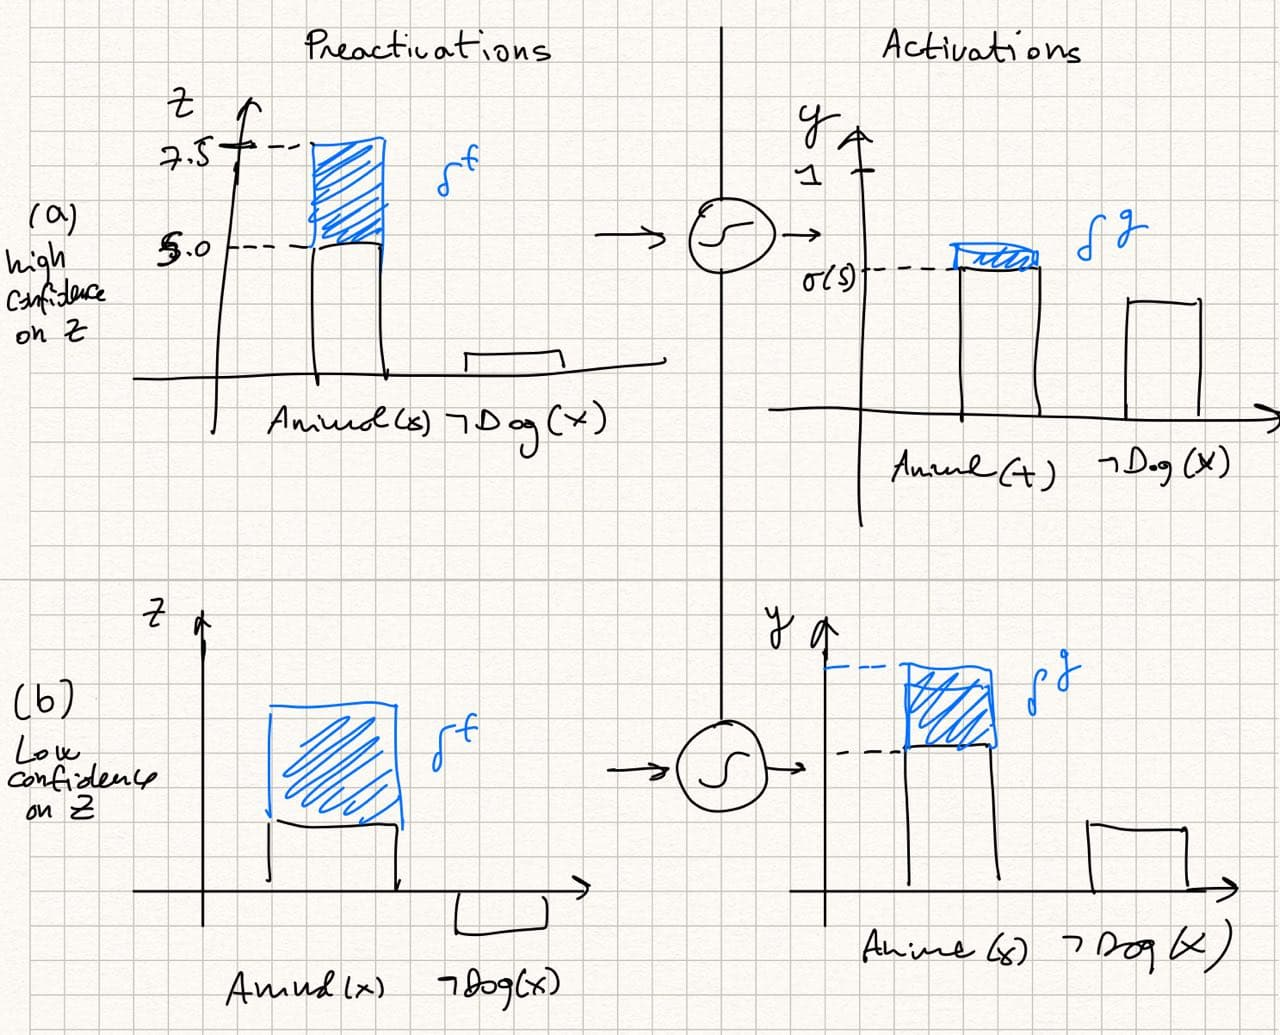
\includegraphics[width=0.8\textwidth]{figures/preac_deltas_example.jpg}
	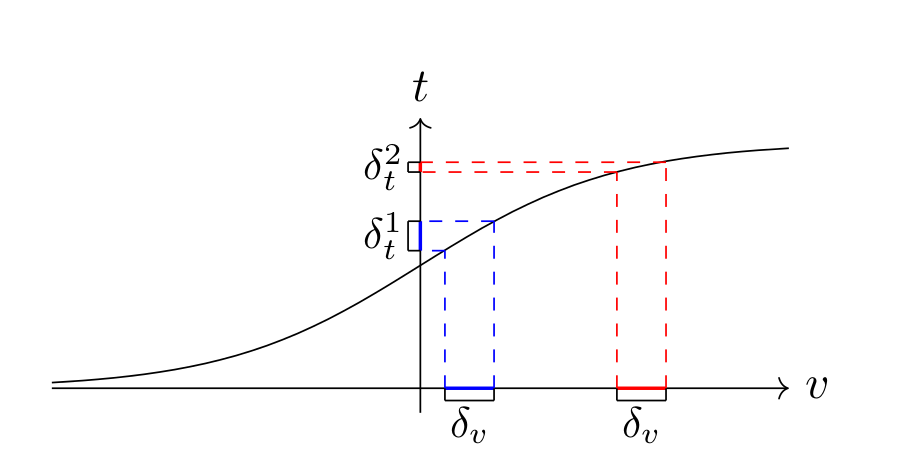
\includegraphics[width=0.5\textwidth]{figures/sigmoid_shape_example.png}
	%TODO: refine this caption
	\caption{This image illustrates the actual deltas produced by KENN, which are the $\delta^f$, opposed to the actual delta produced on the activations, which is $\delta^g$. As we said, $\delta^g$ is not produced directly by the model but it is indirectly \textit{induced} by the application of $\delta^f$ on the preactivations. This also illustrates how, thanks to the shape of the sigmoid activation function, the same delta on the preactivation produces a different delta at the activations level: the closer the preactivations to zero, the highest the modification on the final predictions. }
	\label{fig:preacs_deltas_example}
\end{figure}

As we already mentioned, the minimal TBF directly modeled by KENN is the one we called $\delta^f(z)$. From its definition, we know that the magnitude of the produced delta is determined by the definition of $f$. One of the most important features of KENN is that, by design, it learns to give the proper \textit{importance} to each clause in the base knowledge: this precise feature of the model gives also a way to find such function $f$. Specifically, for each clause $c$ a learnable parameter $w_c$ is defined so that the produced delta for $c$ is:

\begin{equation*}
\delta^{w_c}(z)_i = 
\begin{cases}
w_c \quad &\text{if } i = \arg\max_{j=1}^nz_j \\
0 \quad &\text{otherwise.}
\end{cases}
\end{equation*}

From this definition it's now clear that the function $f$ we were looking for is not actually the same for all the clauses in the base knowledge, but it is defined for each different clause and it's equal to the constant function $f_c(z) = w_c, \quad w_c \in \left[0, \infty\right]$. 
There is one last problem: while it's true that the function $\delta^{w_c}$ is a minimal TBF, the implementation of this kind of functions inside a NN is unfeasible since they are not differentiable. For this reason KENN uses a soft approximation of $\delta^{w_c}$, defined as:

\begin{equation}
\delta_s^{w_c}(z)_i = w_c \cdot \operatorname{softmax}(z)_i = w_c \cdot \frac{e^{z_i}}{\sum_{j=1}^ne^{z_j}}.
\label{eq:soft_approx_delta}
\end{equation}

There are still, however, some steps to describe in order to fully understand how KENN produces a vector of deltas. Recall our notation: we defined with $y \in \mathbb{R}^m$ the vector of predictions from the NN. Specifically, we now define with $y_A$ the truth value relative to $A$, where $A$ is a generic predicate of our language. We also define $z_A=\sigma^{-1}(y_A)$. Now, we note that equation (\ref{eq:soft_approx_delta}), tells us that the produced $\delta$ is always $m$-dimensional, where $m$ is the number of output classes. This however is not desirable: in fact, in general, not all the clauses in our base knowledge contain all the predicates of our language. For example, given $\mathcal{P}=\{A,B,C\}$, the clause $c = A \vee \neg B$ contains only two of the three predicates in the language. Therefore, we would like this specific clause to not modify in any way $z_C$. Another problem is that we don't know how to express the preactivation of a negated literal, i.e. we don't know how to derive $z_{\neg A}$ from $z_A$. In fact, recall that in equation (\ref{eq:lukasiewicz}) we defined the interpretation of a negated predicate, where we knew that the truth values were well defined in the interval $\left[0,1\right]$. Now we are dealing with preactivations, which cannot be considered truth values in the Fuzzy Logic theoretical framework. However, this problem can be easily solved by exploiting the following property of the sigmoid activation function:

\begin{equation*}
1 - \sigma(x) = \sigma(-x).
\end{equation*}

Now it's easy to see that, since $y_{\neg A} = 1 - y_A$, we can define:

\begin{equation*}
z_{\neg A} = -z_A.
\end{equation*}

Notice that we are not introducing any new concepts: instead we are just redefining quantities that were already mentioned at the activation level, to the preactivation level. %TODO Maybe remove this sentence
We finally define $z_c = \left(z_{l_1}, \dots, z_{l_k}\right)$ for every clause $c := \bigvee_{i=1}^k l_i$ of the knowledge. We refer to the process of transforming from $z$ to $z_c$ as the \textit{selection} step. This new vector contains only the preactivations of literals present in $c$, and is the one that we actually want to use to produce the delta relative to clause $c$. Now, let $\mathcal{K}$ be the set of clauses in our knowledge, and $\{w_c\}_{c\in\mathcal{K}}$ their corresponding weights. For every clause $c\in \mathcal{K}$ we want to obtain a new delta, namely $\delta^c \in \mathbb{R}^m$, which contains one value for each predicate in the clause and is defined as follows:

\begin{equation}
\delta_{A}^{c}= \begin{cases}\delta_{s}^{w_{c}}\left(z_{c}\right)_{A} & \text { if } A \in c \\ -\delta_{s}^{w_{c}}\left(z_{c}\right)_{\neg A} & \text { if } \neg A \in c \\ 0 & \text { otherwise }\end{cases}, \quad \forall A \in \mathcal{K}
\label{eq:delta_c}
\end{equation}

This newly defined delta, $\delta^c$, will be the delta obtained from clause $c$ and will be summed to $z$ to obtain the updated prediction. More specifically:

$$y' = \sigma(z + \delta^c)$$

\begin{figure}[h!]
	\centering
	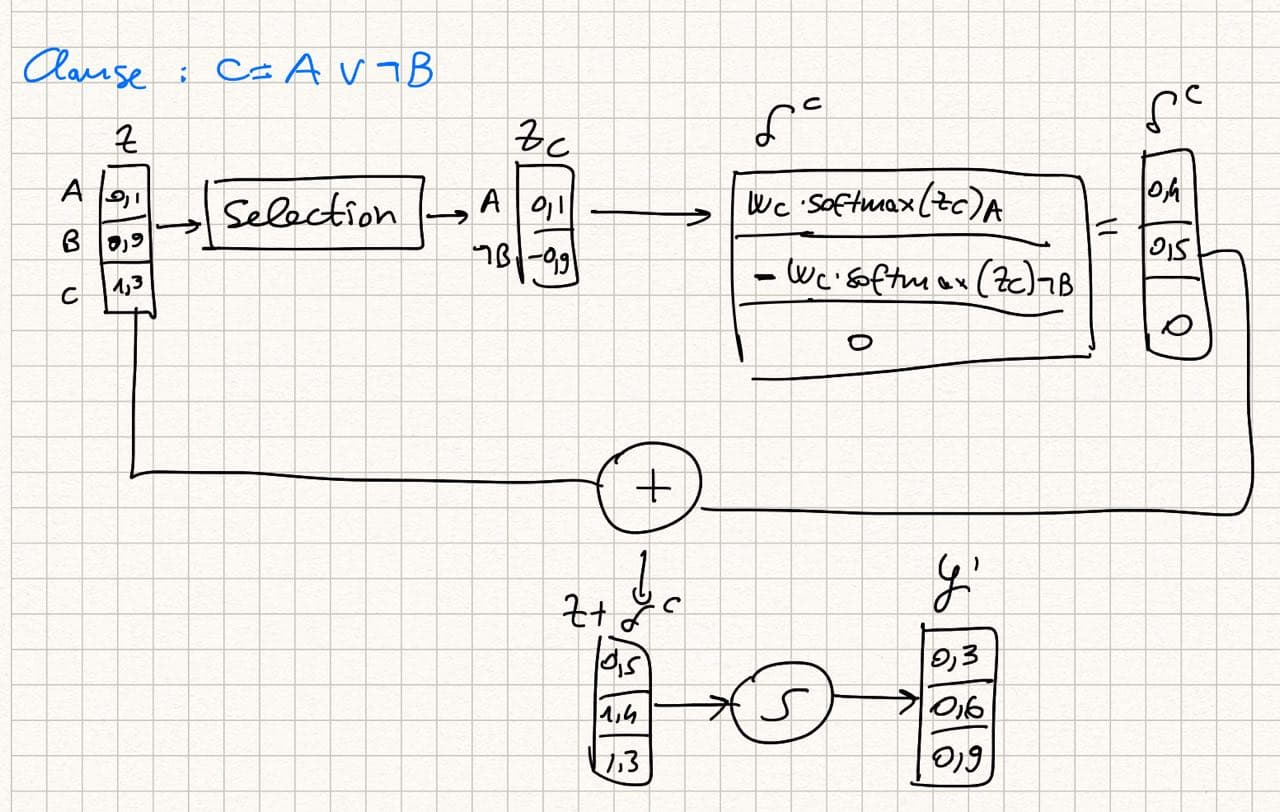
\includegraphics[width=0.8\linewidth]{figures/delta_single_clause.png}
	\caption{Summary of all the steps needed to produce $\delta^c$, the vector of deltas derived from a single clause. We refer to this process as \textit{clause enhancement}.}
	\label{fig:delta_single_clause}
\end{figure}


\subsection{Increasing the satisfaction of the Knowledge}
In the previous section we found out how KENN produces a vector of changes $\delta$ to be applied to the original NN predictions, but only considering a single clause. That would suffice in the cases where the knowledge is constituted only by a single clause, but in real applications a higher number of logical rules will be desirable. Therefore, the next and final problem is to understand how KENN takes all the deltas from all the clauses and produces a single vector of changes. This particular step of aggregation is critical, as it constitutes one of the best features of KENN, but at the same time one of its bigger inaccuracies. This is because, to aggregate the contributions from all the clauses $c \in \mathcal{K}$, KENN just sums the contributions. Specifically, the final prediction is defined as follows:

\begin{equation}
\label{eq:deltas_sum}
y'=\sigma(z + \sum_{c\in\mathcal{K}}\delta^c).
\end{equation}
This particular choice makes KENN really fast at inference and learning time, increasing scalability. At the same time, though, this makes the risk of inconsistencies higher. For example, the same predicate can appear negated in one clause, and not negated in another clause: in this way the delta for the first one will be negative while it will be positive for the second one. In this way, the two deltas may cancel out rendering the contributions of the two clauses less effective.


\section{KENN Architecture}
In this section we present the architecture of the KENN layer in details. To be more precise, the architecture we are about to describe is valid only for unary predicates, meaning that only unary clauses will work as base knowledge. In the next section (ref TODO) we will also see that KENN is capable of dealing with binary clauses, but that will require a modification of the architecture. 

As described above, the core functionality of KENN is the \textit{clause enhancement}, i.e. the creation of a vector $\delta$ which, summed to the vector of predictions $y$, produces a modified vector of predictions $y'$ which increases the truth value of the relative clause. The architecture that takes care of this task is the Clause Enhancer (CE): this submodule takes in input the full vector of preactivations from the original NN and computes the vector of deltas $\delta^c$ described in equation (\ref{eq:delta_c}). For each clause in the base knowledge, a CE will be instantiated. The details of the architecture of the CE are described in Figure \ref{fig:CE}.

\begin{figure}
	\centering
	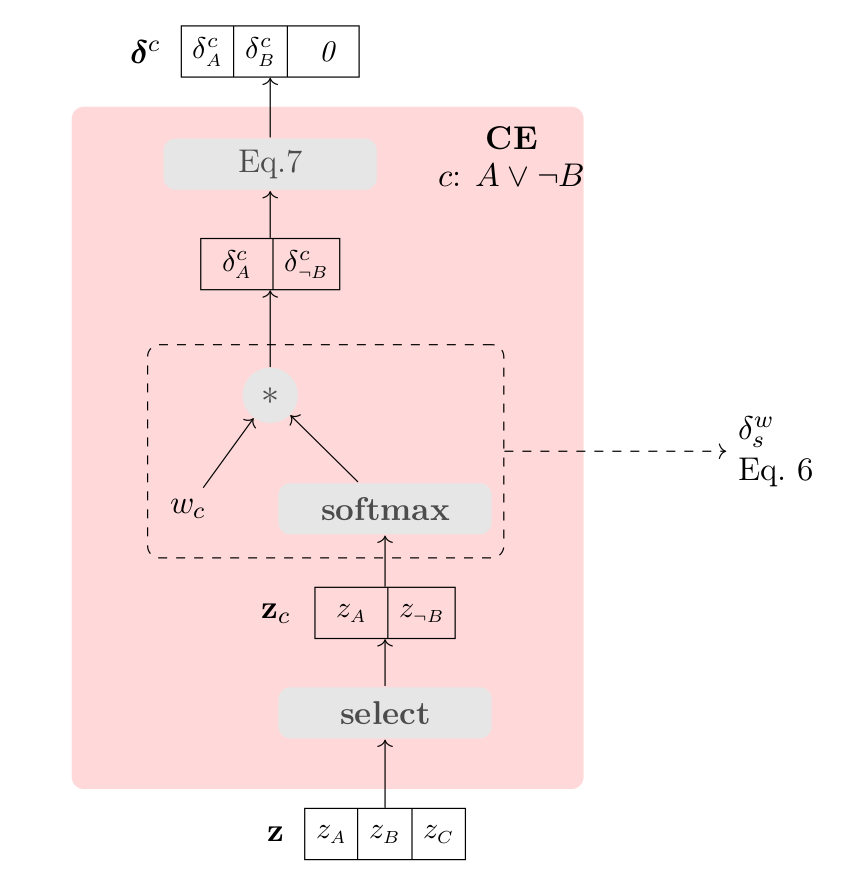
\includegraphics[width=0.8\linewidth]{figures/CE.png}
	%TODO: fare bene la caption quando avrò l'immagine giusta
	\caption{Detailed depiction of the Clause Enhancer for the clause.... todo}
	\label{fig:CE}
\end{figure}

The CE performs the following operations:
\begin{enumerate}
	%TODO: refine the steps
	\item takes the preactivations...
	\item perform the select step..
	\item creates delta according to eq...
	\item transforms back from zof literals to z of predicates ...
\end{enumerate}

Once the delta for each clause ($\delta^c$) is produced by its corresponding CE, the next step is to aggregate all the deltas by summing them. The module that performs this operation is called the \textit{Knowledge Enhancer} (KE), which is shown in Figure \ref{fig:KE}. More specifically, the KE performs the following operations:
\begin{enumerate}
	\item Takes as inputs all the $\delta^c$ for each clause $c$ in the knowledge and sums them. 
	\item It sums the obtained delta with the original preactivations 
	\item Applies the sigmoid activation function.
\end{enumerate}

\begin{figure}
	\centering
	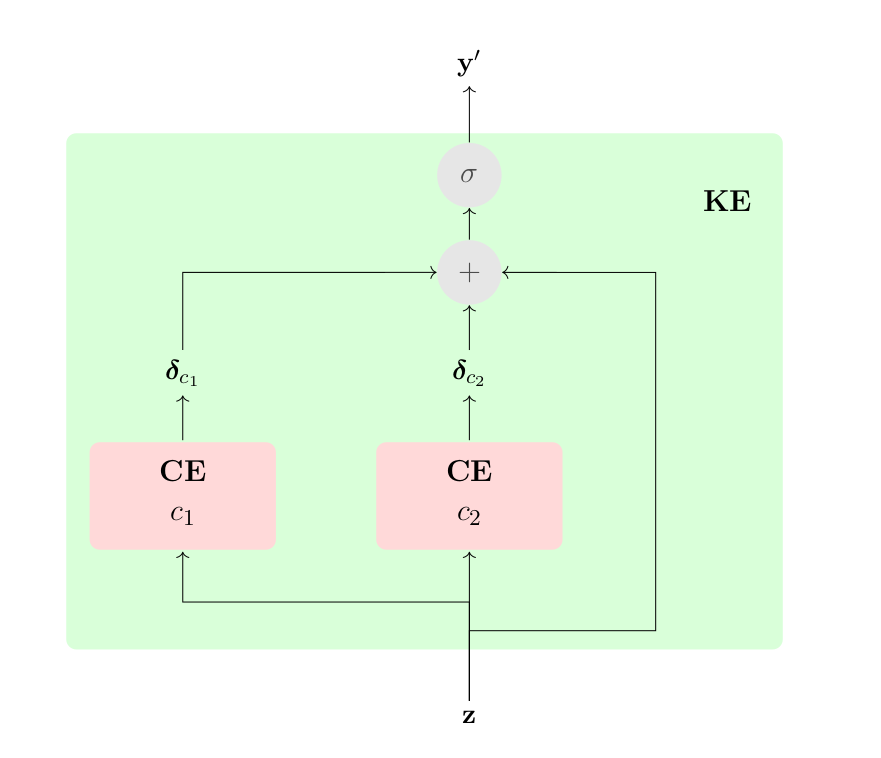
\includegraphics[width=0.8\linewidth]{figures/KE.png}
	%TODO also refine here
	\caption{The KE architecture... todo}
	\label{fig:KE}
\end{figure}

 These steps produce the final vector of modified predictions $y'$. Notice that the KE is just the implementation of equation (\ref{eq:deltas_sum}).
 
 \section{KENN for relational data}
 
 
 \begin{figure}
 	\centering
 	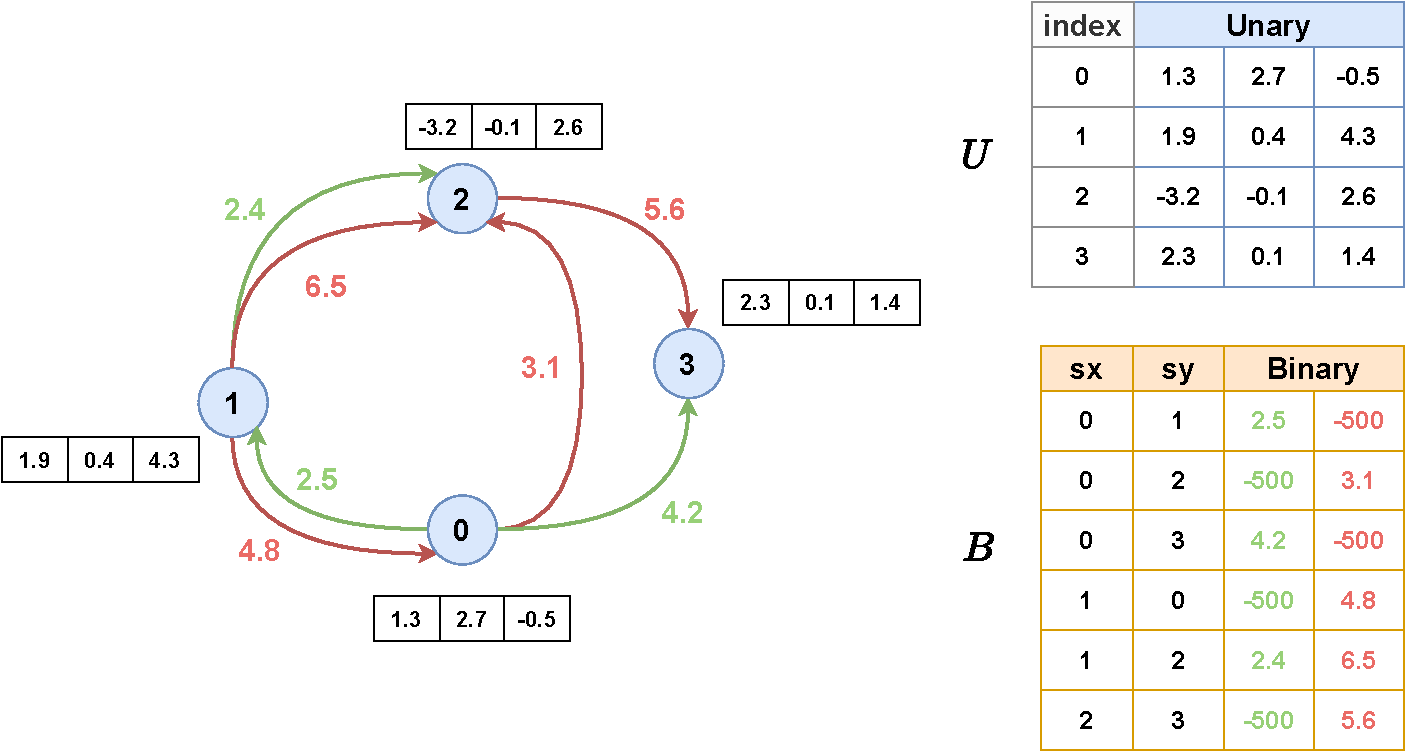
\includegraphics[width=\linewidth]{figures/kenn_relational_representation.pdf}
 	\caption{Representation of relational data inside KENN}
 	\label{fig:KENNrelationalrepr}
 \end{figure}
 
 
 \section{Related Work}
 Here we report different approaches for injecting logical knowledge inside neural networks....INTRO TODO %TODO: fai introoo
 
 % TODO: STUDIARE BENE DA PAPER KENN
 %TODO possibili intro...
% In spite of the amazing results obtained by deep learning in
% many applications, a real intelligent behavior of an agent acting in a
% complex environment is likely to require some kind of higher-level symbolic
% inference. Therefore, there is a clear need for the definition of a general and
% tight integration between low-level tasks, processing sensorial data that
% can be effectively elaborated using deep learning techniques, and the logic
% reasoning that allows humans to take decisions in complex environments. (from Lyrics paper)
 
 % altra survey interessante con info: https://arxiv.org/pdf/2003.08316.pdf
% Interesting pieces from besold et al (neural symbolic integration paper): intuitive motivation for NSI:
% in neural computing it is assumed that the mind is an emergent porperty of the brain, and that computational cognitive modelling can lead to valid theories of cognition and offer an understanding of certain cognitive processes (sun 2009)
% 
% the Connectionism model should ffer an appropriate representational language for artificial intelligence; in particular this kind of model can replicate parallelism and adaptive learning, present in neuralnetworks: this assures the effectivenes and robusteness of the system, to deal with commonsense knowledge.. all this to say that a purely symbolic approach would not be sufficient (as argued by Valiant 2008 ).
% 
% On the other hand, logic is firmly established as a fundamental tool in the modelling of thought and behaviour... We have to concile these two areas.
% 
% However when building models that combine both learning and reasoning, one has to conciliate the methodologies of distinct areas (basically statistics vs logic), in order to combine respective advantages and circumvent the shortcomings and limitations of each other. This problem has been identified as a key research challenge and fundamental problem in computer science... (Valiant 2003)
% 
% The goals of NSI are to provide a coherent, unifying view for logic and connectionsim, to contribute to the modelling and understanding of cognition and, thereby, behavior, and to produce better computational tools for integrated machine learning and reasoning. In a nutshell: encompasses the high level integration of cognitive abilities and the study of how the brain makes a mental model... at the computational level, it addresses the study of the integration of logic, probabilities, and learning, and the development of new models of computation combining robust learning and efficient reasoning.
 
 So as we can see NSI is a really vast area of research. In our case we are interested in the usage of knowledge inside a neural network. Authors in \cite{daniele2019kenn,serafini2016logic} subdivide NSI sytstems into three main groups, based on their different objectives:
 \begin{enumerate}
 	\item \textbf{Differentiable Reasoning }: ... (capire bene cosa significa "reasoning")
 	\item \textbf{Inductive Logic Programming} : here the goal is to extract logical knowledge from data, or to refine an existing one
 	\item \textbf{Knowledge Guided Learning}: here the goal is Learning in classical ML sense, and Knowledge has the role of supervisor, meaning that the machine should learn according to the base knowledge.
 \end{enumerate}
 
 We are interested in the third class of models, the one where KENN belongs. The objective is to improve the performance of a neural network model, by providing a Prior Knowledge which is expressed in terms of logical formulas. At present, two main ways of injecting knowledge inside NN have been employed. The first one involves the usage of a regularization term in the loss function. Indeed, logical rules can be interpreted as costraints for the weights in the learning process; in machine learning, the natural way to introduce costraints in learning is to add a penalization term in the loss function, which represents in some way the satisfaction of the logical rules. The second approach, adopted by KENN, is to directly modify the network architecture: in this way, logical rules are not enforced by external penalizations but are already present in the network topology ... (riscrivere bene)
 
 \subsection{Regularization Approaches}
 Logic Tensor Networks, Semantic based regularization....
 
 \subsubsection{Logic Tensor Networks}
 %TODO: è  ancora una bozza.. riscrivere bene...
 Logic Tensor Networks (LTN) \cite{serafini2016logic} is a notable example of methods capable of integrating logical knowledge inside neural networks by directly modifying the loss function. To do this, the authors define a differentiable first-order logic language called Real Logic, with which they manage to represent common deep learning tasks, such as clustering, multi-label classification, relational learning, query answering, semi-supervised learning, regression and embedding learning. 
 %LTN can also perform reasoning, which is the task of verifying if a formula is a logical consequence of another formula. 
 In simple terms, the role of Real Logic is to act as a bridge between the purely symbolic world of logic, and the sub-symbolic world of neural systems. We give a brief summary of the core definitions in Real Logic, in order to understand how learning is possible.
 
 Real Logic is defined over a first order language $\mathcal{L}$ with a signature containing a set of constant symbols (or objects) $\mathcal{C}$, a set of variable symbols $\mathcal{X}$, a set of functional symbols $\mathcal{F}$ and a set of relational symbols (or predicates) $\mathcal{P}$. We refer to the set $\mathcal{S} = \mathcal{C} \cup \mathcal{X} \cup \mathcal{F} \cup  \mathcal{P}$ as the set of symbols of $\mathcal{L}$. Each symbol of the language can belong to different domains (i.e. can be of different types): for example the constant $c_1 \in \mathcal{C}$ can represent a specific person, while the constant $c_2 \in \mathcal{C}$ can represent a specific city. The same concept applies to functions and predicates. To represent the domain of each symbol, it is assumed that there exists a non-empty set $\mathcal{D}$, containing all the domains, which are in turn symbols. Then, to properly assign each symbol to its corresponding domain, the functions $\mathbf{D}, \mathbf{D_{in}}$ and $\mathbf{D_{out}}$ are defined:
 
 \begin{equation*}
 \mathbf{D}: \mathcal{X} \cup \mathcal{C} \rightarrow\mathcal{D}
 \qquad \qquad
 \mathbf{D_{in}}: \mathcal{F} \cup \mathcal{P} \rightarrow\mathcal{D^*}
 \qquad \qquad 
 \mathbf{D_{out}}: \mathcal{F} \rightarrow\mathcal{D},
 \end{equation*}
 
 where $\mathcal{D^*}$ is the set of all finite sequences of symbols in $\mathcal{D}$.
 %The set of terms of the language $T$ is recursively defined, to be the smallest set such that...
 The point where the symbolic language meets the subsymbolic world of neural networks is in the definition of grounding, which is the process in which each symbol is given its numeric representation. Indeed, in Real Logic, each domain is interpreted as sets of tensors in the real field. In the same way, each constant, variable and term of the language is interpreted as a tensor of real values, and function symbols are interpreted as functions between tensors. Predicates, are interpreted as functions that map tensors into the interval$[0,1]$. So, given $s$ any symbol of $\mathcal{L}$, its grounding is denoted as $\mathcal{G}(s)$. 
 %By defining how to apply the grounding for each symbol of $\mathcal{L}$, semantic of $\mathcal{L}$. 
 The authors then define how to compute the grounding of formulas, by using the semantics of first-order fuzzy logic. 
 The way in which learning becomes possible is by defining parametric definition of grounding for symbols: given a symbol $s$, the parametric grounding of $s$ is a grounding which is not known in advance, and can be computed exclusively by knowing a set of parameters. It is denoted as $\mathcal{G}(s|\theta_s)$, where $\theta_s$ is the set of parameter values that uniquely determines the value of the grounding. It's interesting to note that, based on what kind of symbol we are learning the grounding for, one can identify a corresponding task in machine learning:
 \begin{itemize}
 	\item If $s \in \mathcal{C}$, corresponds to learning an embedding;
 	\item If $s \in \mathcal{F}$, it corresponds to learning generative models, or regression tasks;
 	\item If $s \in \mathcal{P}$, it corresponds to learning a classification task.
 \end{itemize}
 
 \subsubsection{Semantic Based Regularization}
 Semantic Based Regularization (SBR) is a general learning framework designed to integrate domain specific background knowledge in the form of first-order logic (FOL) clauses. To enforce the satisfaction of all the clauses, SBR introduces special regularization terms in the loss function, which represent the satisfaction of the knowledge. Specifically, given a background knowledge represented by set of $H$ clauses, the satisfaction of the $h$-th clause can be represented by the quantity denoted by $0 \leq \phi_h(f) \leq 1$, where $f$ is the vector function learned by the model. From here, the regularization term to be added to the loss function is defined as
 
 $$ \sum_{h=1}^H \lambda_h(1 - \phi_h(f)), $$
 
 where $\lambda_h$ is the weight associated to the $h$-th constraint. A higher value of $\lambda_h$ will increase the cost of not satisfying the constraint, meaning that the importance of the corresponding rule will increase. The conversion of FOL clauses into differentiable functions is made possible by considering fuzzy generalizations of FOL logic, similarly to how it is done in KENN.
% TODO: la cit non va proprio qui.. 
 . This is a natural approach for machine learning tasks, but a major disadvantage over KENN is that, since the clause weights are introduced at the level of the loss function, those cannot be learned and are required to be known in advance. This, of course, is unlikely to happen in real scenarios and it is much more desirable to learn the weights together with the other learnable parameters of the model.
 
 \subsection{Model Based Approaches}
 
 \section{Experiments}
 
In this section we describe in detail the experiments performed with KENN. We tested the ability of KENN of working with relational data, in the context of Collective Classification~\cite{sen2008collective}, both with the inductive and transductive learning paradigm. 

\begin{definition}[Collective Classification]
Consider a directed graph, consisting in a set of nodes $V$ and a set of edges $E$. Each $v \in V$ is described with a vector of features $x\in \mathbb{R}^n$ and belongs to one of $k$ classes $\{\omega_i\}_{i=1}^k$. The set of nodes $V$ is further divided in two subsets of nodes: $X$, the set of nodes for which the correct label is known (Training Set), and $Y$, the set of nodes for which it is unknown (Test Set). The task of Collective Classification is to correctly predict the labels of nodes in $Y$, given the feature vectors of $X$ and the topology structure determined by $E$. 
\end{definition}

Based on how the edges from $E$ are split between Training and Test set, a different learning paradigm is defined:

\begin{itemize}
	\item \textbf{Inductive Learning}: two separate graphs are used, $G_x = (X,E_x)$ for training and $G_y = (Y, E_y)$ for testing, where $E_x = \{(u,v) | u,v\in X\}$ and $E_y = \{(u,v) | u,v\in Y\}$. In other words, the edges of nodes between train and test set are not considered.
	\item \textbf{Transductive Learning}: in the training graph, also edges connecting training and test data are retained. This means that the model can use additional information, in the form of connections between test and training data, even during training.
\end{itemize}

We also provide a comparison of our results with the ones from SBR and RNM, reported on \cite{marra2020relational}, on the same dataset and tasks. 

\subsection{Citeseer Dataset}

The experiments were conducted on the Citeseer Dataset \cite{lu2003link}: it consists in a citation network with $4732$ citations (directed links) between $3312$ scientific publications (nodes), belonging to 6 different classes which represent the topic of the paper. Each node in the dataset is represented by a $0/1$ valued feature vector, where each entry indicates the absence or presence of the corresponding word in the dictionary, which is constituted by $3703$ unique words.

\subsection{The Prior Knowledge}

The knowledge that we want to use in order to improve the predictions from the NN is the intuitive fact that, if a paper cites another paper, it is probably true that they are of the same topic. If we denote with $T_i(x)$ the truth value that node $x$ belongs to the $i$-th output class, this fact can be encoded in terms of a logical clause as follows:

$$\forall x \forall y \quad T_i(x) \wedge \operatorname{Cite}(x, y) \rightarrow T_i(y), \quad i=1,\dots,6$$

meaning that the this clause is repeated one time for each different output class. Inside KENN, this clause is represented as a disjunction of literals as follows:

$$\forall x \forall y \quad \neg T_i(x) \vee \neg \operatorname{Cite}(x,y) \vee T_i(y), \quad i=1,\dots,6 $$


\subsection{Results}

In Table \ref{tab:resultsinductive} we report the results of the experiments for the inductive case. The accuracies for KENN are the mean of $500$ different runs on different randomly extracted splits.
In Table \ref{tab:resultstransductive} the results for the transductive case are reported.
\begin{table}[h]
	\caption{Results of kenn experiments for the inductive case....}
	\label{tab:resultsinductive}
	\centering
	\begin{tabular}{c|lll|ll} 
	\% training & NN & SBR & RNM & NN & KENN \\
	\hline 
	\rule{0pt}{3ex}    $10$ & $0.645$ & $0.650$ & $\mathbf{0 . 6 8 5}$ & $0.544$ & $0.601$ \\
	& & $(+0.005)$ & $(+0.040)$ & & $\mathbf{(+0.048)}$ \\
	$25$ & $0.674$ & $0.682$ & $\mathbf{0 . 7 0 9}$ & $0.629$ & $0.671$ \\
	& & $(+0.008)$ & $(+0.035)$ & & $\mathbf{( + 0 . 0 4 1 )}$ \\
	$50$ & $0.707$ & $0.712$ & $\mathbf{0 . 7 2 6}$ & $0.680$ & $0.714$ \\
	& & $(+0.005)$ & $(+0.019)$ & & $(+\mathbf{0 . 0 3 4 )}$ \\
	$75$ & $0.717$ & $0.719$ & $0.726$ & $0.733$ & $\mathbf{0 . 7 5 4}$ \\
	& & $(+0.002)$ & $(+0.009)$ & & $\mathbf{( + 0 . 0 2 1 )}$ \\
	$90$ & $0.723$ & $0.726$ & $0.732$ & $0.759$ & $\mathbf{0 . 7 6 8}$ \\
	 & & $(+0.003)$ & $(+0.009)$ & & $\mathbf{( + 0 . 0 1 0 )}$\\	
	\hline \hline
\end{tabular}
\end{table}

\begin{table}[h]
	\caption{Results of kenn experiments for the transductive case....}
	\label{tab:resultstransductive}
	\centering
\begin{tabular}{c|lll|ll} 
	\% training & NN & SBR & RNM & NN & KENN \\
	\hline 
	\rule{0pt}{3ex} $10$ & $0.640$ & $0.703$ & $\mathbf{0 . 7 0 8}$ & $0.544$ & $0.652$ \\
	& & $(+0.063)$ & $(+0.068)$ & & $(+\mathbf{0 . 1 0 8 )}$ \\
	$25$ & $0.667$ & $0.729$ & $\mathbf{0 . 7 3 5}$ & $0.629$ & $0.702$ \\
	& & $(+0.062)$ & $(+0.068)$ & & $(+\mathbf{0 . 0 7 3})$ \\
	$50$ & $0.695$ & $0.747$ & $\mathbf{0 . 7 5 3}$ & $0.680$ & $0.744$ \\
	& & $(+0.052)$ & $+0.058)$ & & $(+\mathbf{0 . 0 6 5 )}$ \\
	$75$ & $0.708$ & $0.764$ & $0.766$ & $0.733$ & $\mathbf{0 . 7 8 8}$ \\
	& & $(+0.056)$ & $(+\mathbf{0 . 0 5 8})$ & & $(+0.055)$ \\
	$90$ & $0.726$ & $0.780$ & $0.780$ & $0.759$ & $\mathbf{0 . 8 0 8}$ \\
	& & $\mathbf{( + 0 . 0 5 4 )}$ & $\mathbf{( + 0 . 0 5 4 )}$ & & $(+0.049)$ \\
	\hline \hline
\end{tabular}
\end{table}

\begin{figure}
	\centering
	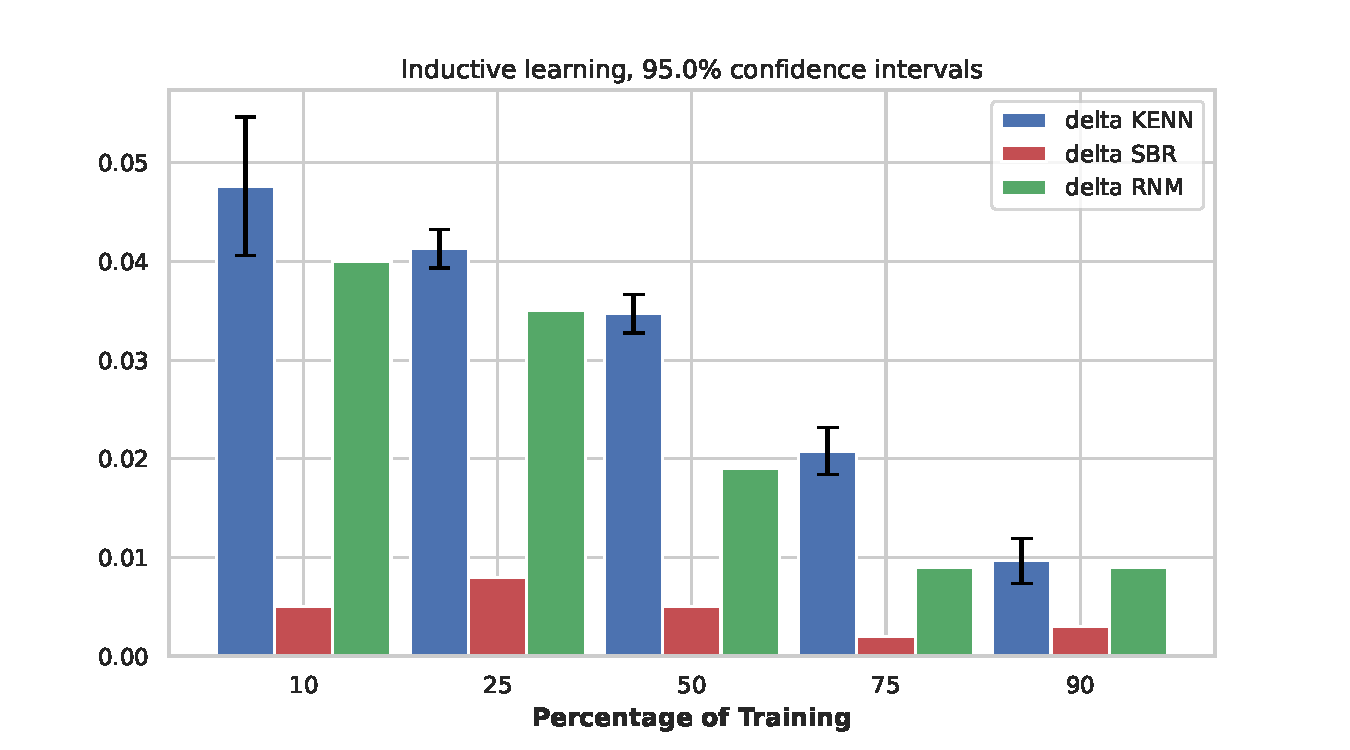
\includegraphics[width=0.9\linewidth]{figures/deltas_inductive.pdf} 
		\caption{Deltas for the inductive learning task. $95\%$ confidence intervals.}
\end{figure}

\begin{figure}
	\centering
	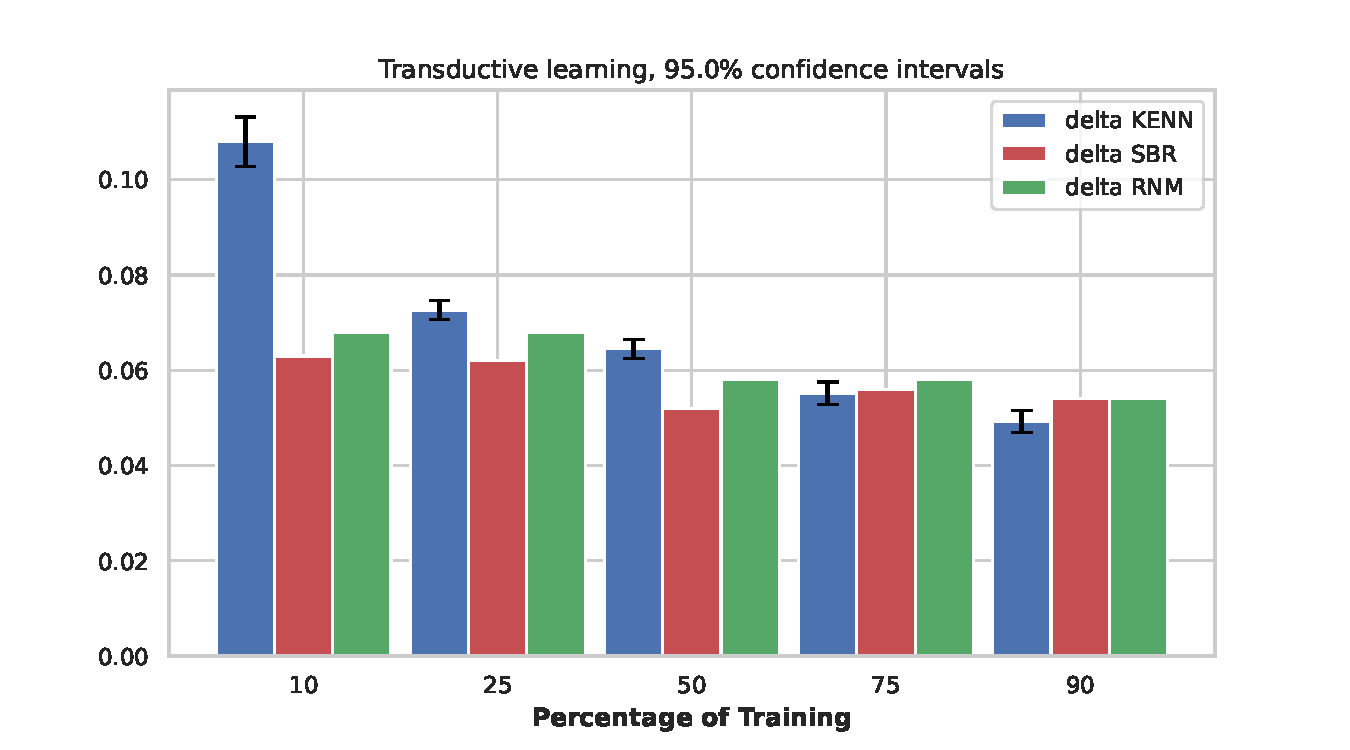
\includegraphics[width=0.9\linewidth]{figures/deltas_transductive.pdf}
		\caption{Deltas for the transductive learning task. $95\%$ confidence intervals.}
\end{figure}

\begin{figure}
	\centering
	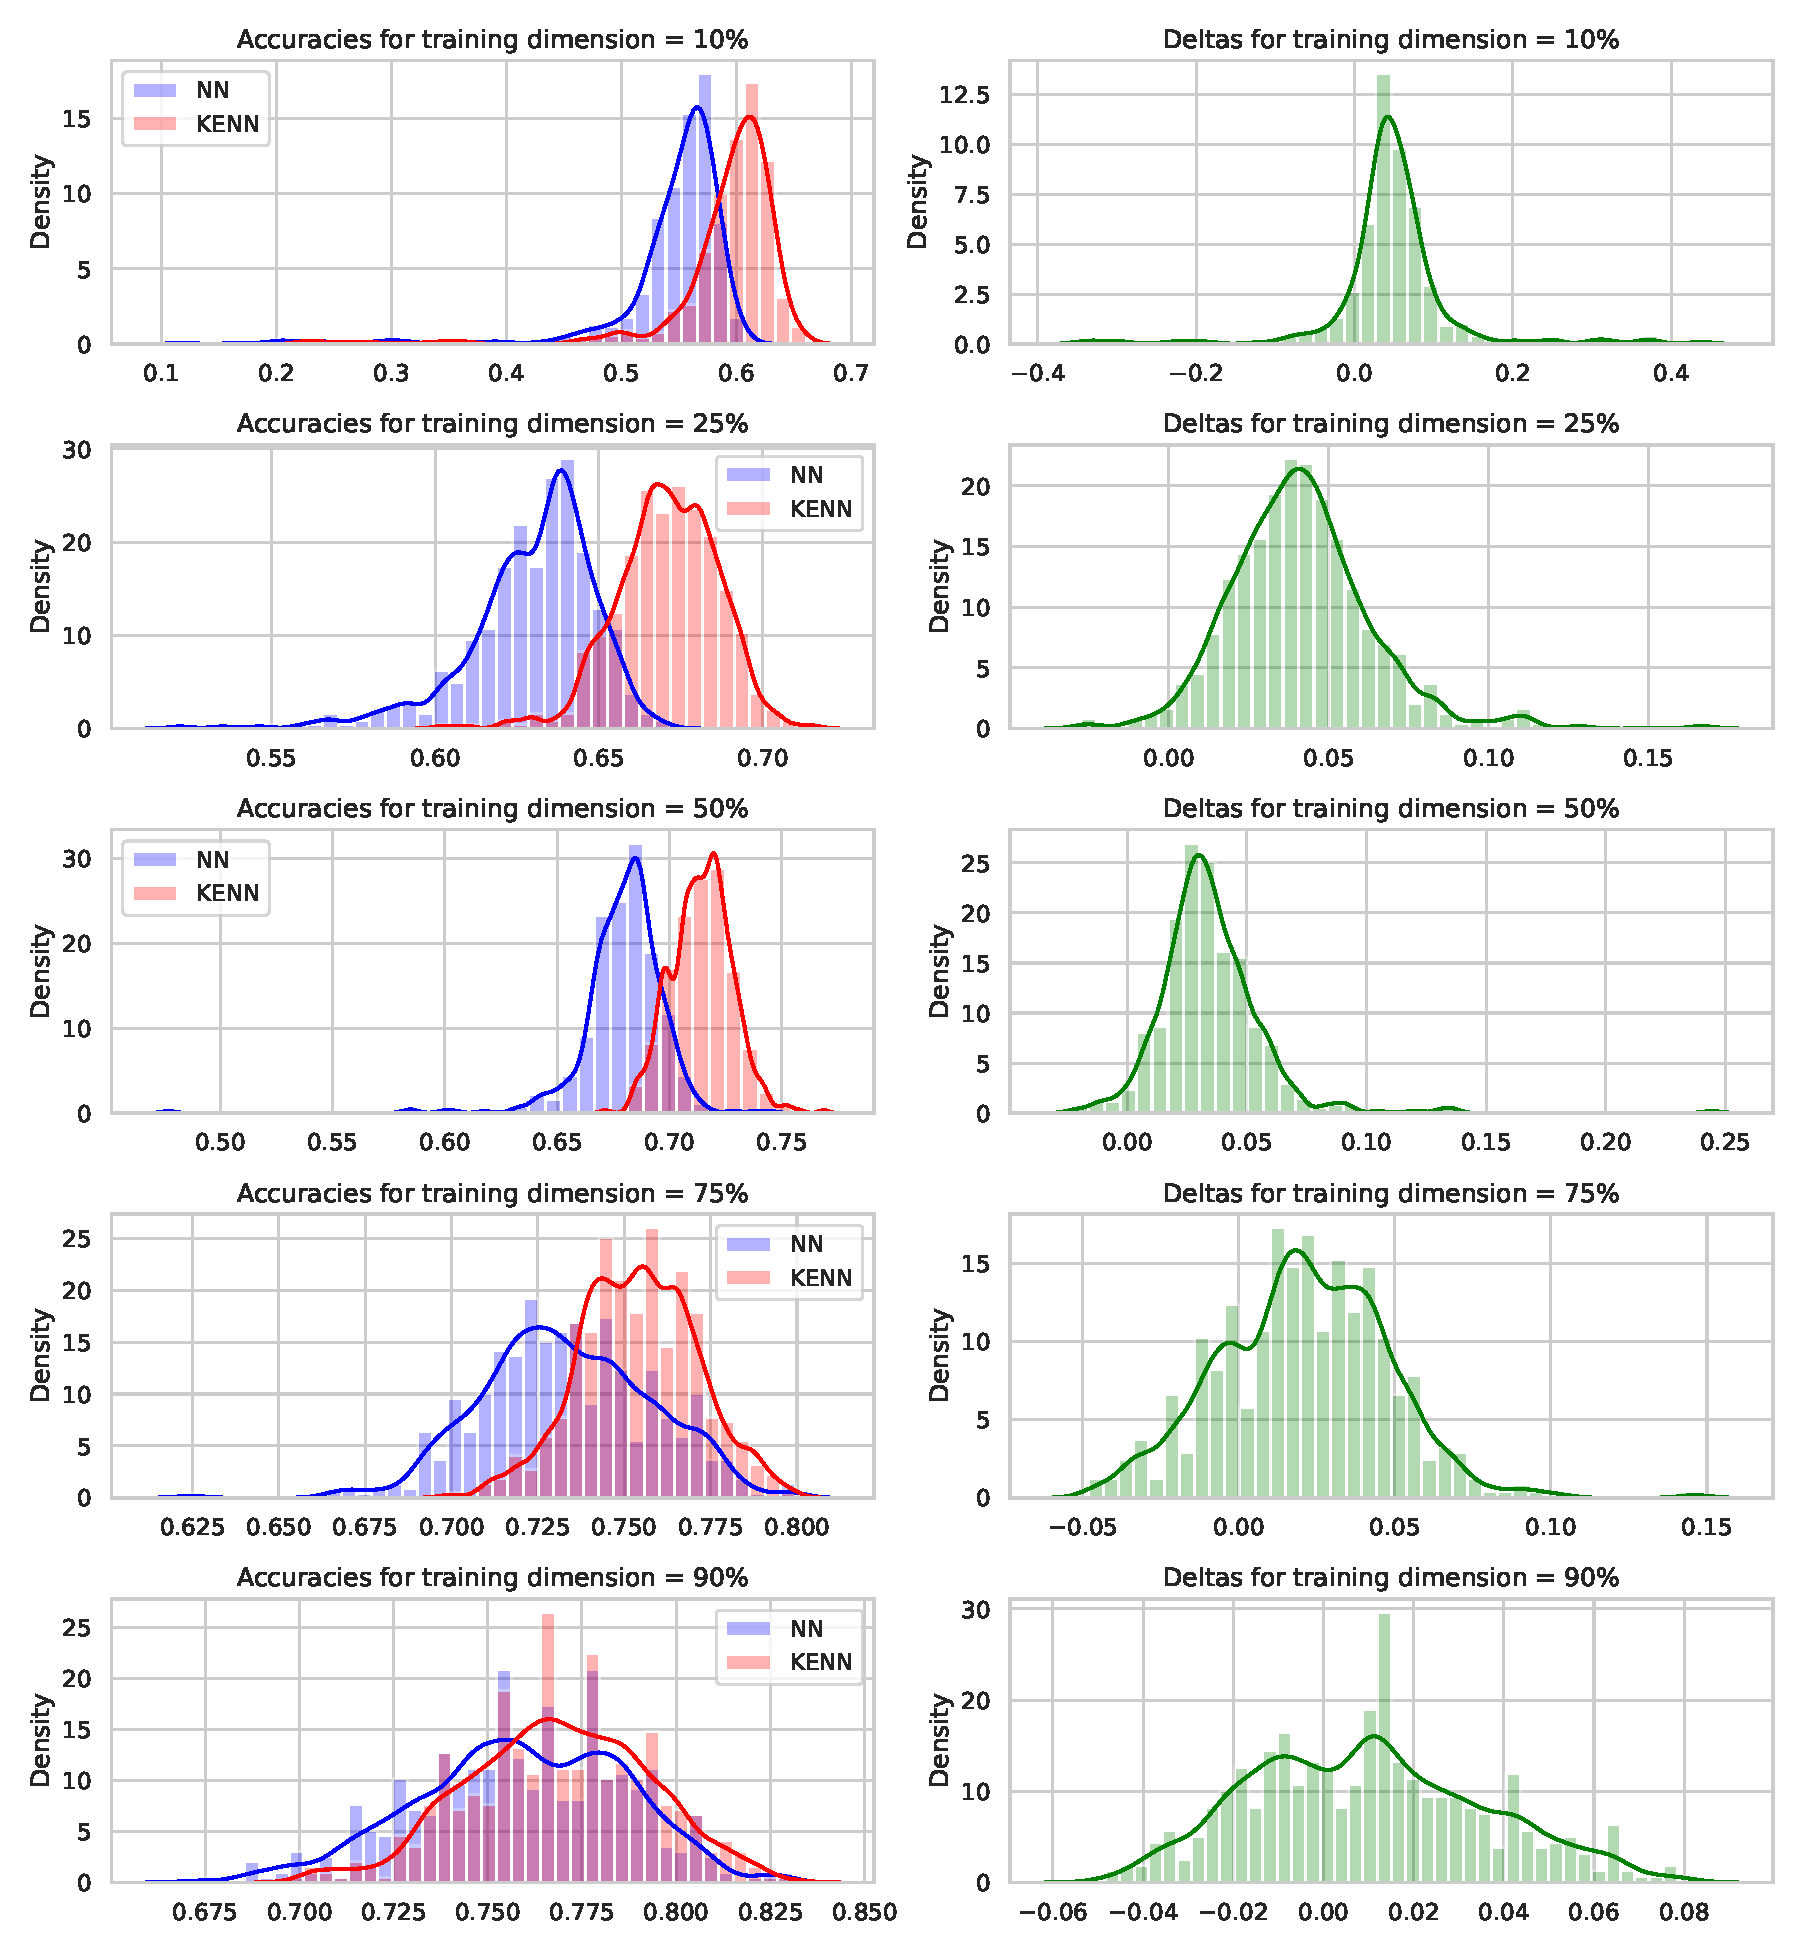
\includegraphics[width=0.95\linewidth]{figures/histograms_inductive.pdf}
	\caption{Histograms showing the distribution of the accuracies for all the different $500$ runs, for the inductive case. On the left, the accuracies of the base NN vs accuracies of KENN. On the right the distribution of the difference between the NN accuracy vs KENN accuracy.}
\end{figure}

\begin{figure}
	\centering
	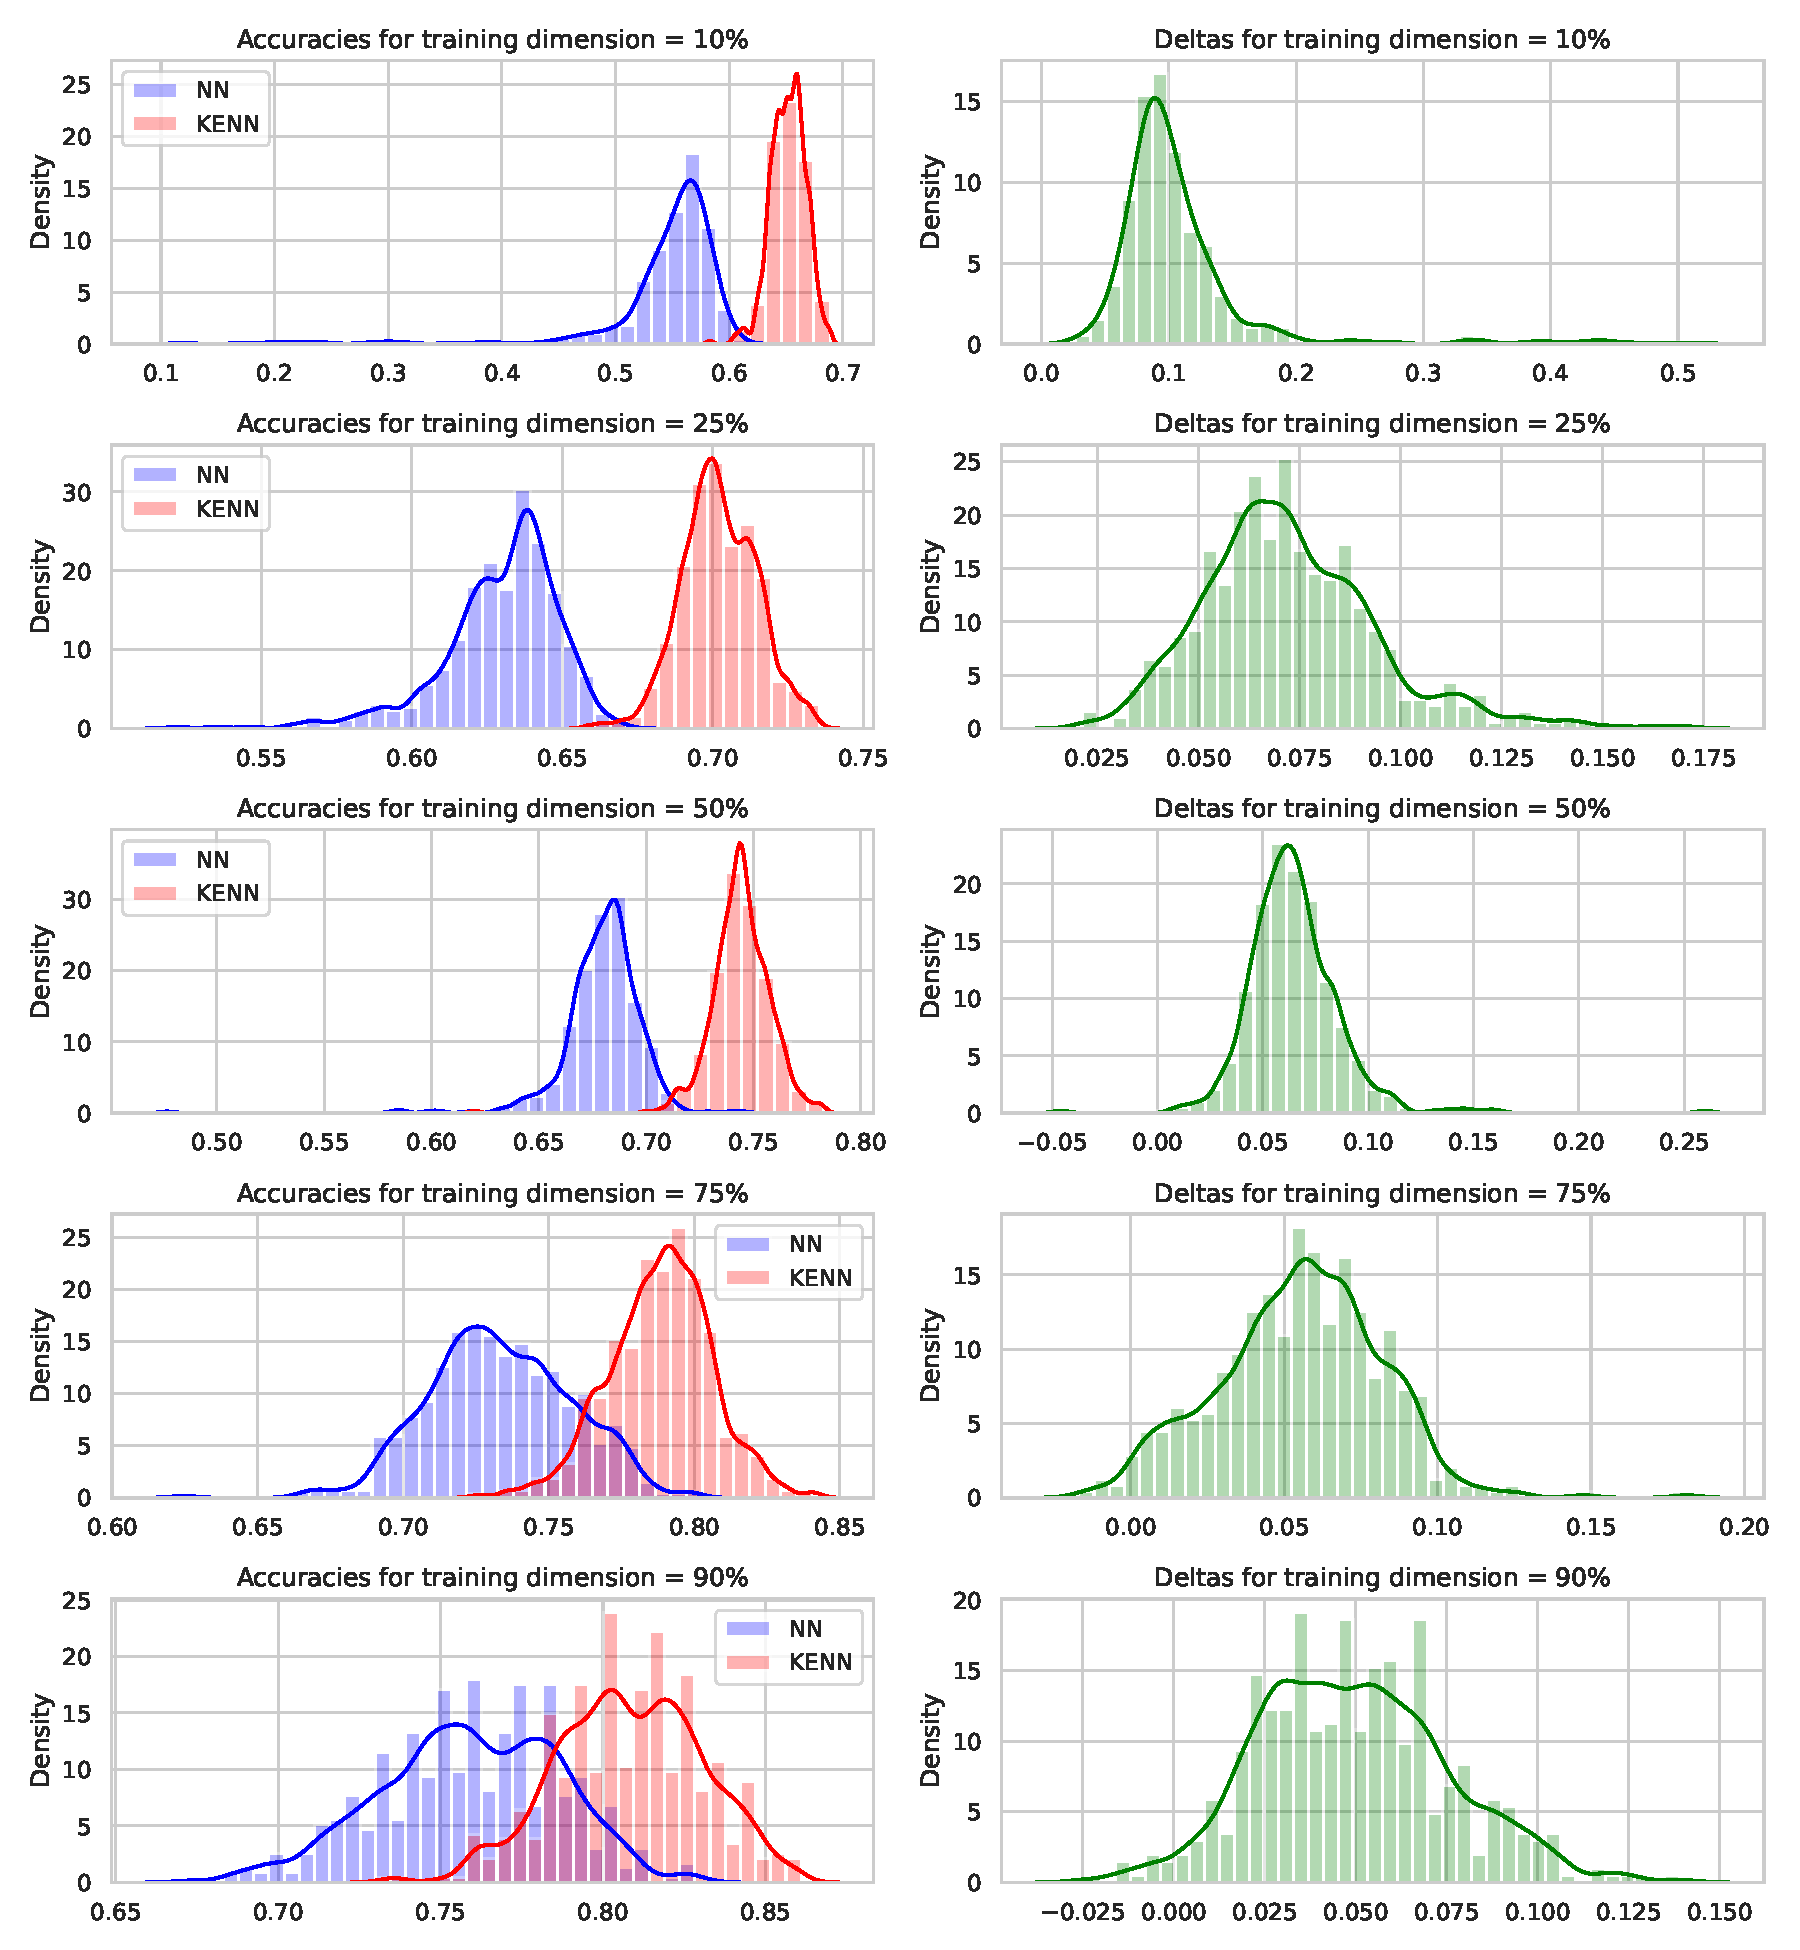
\includegraphics[width=0.95\linewidth]{figures/histograms_transductive.pdf}
	\caption{Histograms showing the distribution of the accuracies for all the different $500$ runs, for the transductive case. On the left, the accuracies of the base NN vs accuracies of KENN. On the right the distribution of the difference between the NN accuracy vs KENN accuracy.}
\end{figure}





\subsection{Clause Weights and satisfaction of the rules}
 
 \section{Explainability in KENN}
%TODO:
% In che modo KENN è un modello explainable/interpretable.
% Prima fare qualche collegamento con quanto visto nel capitolo dell'explainability...
% \begin{enumerate}
% 	\item clause weights -> quanto le clausole influiscono sulle predizioni
% 	\item ispezionare i delta permette di vedere direttamente come è stata modificata una predizione e perché;
% 	\item possibilità di definire metriche (rank by improvement etc) che permettono di capire bene quali predizioni sono state migliorate, quali peggiorate, e a causa di quale clausola.
% 	\item Interpretability: si può capire come KENN impari i clause weights e quanto è legato alla "verità di una clausola"-> correlazione tra clause compliance e clause weights.
% \end{enumerate}

